\documentclass[aspectratio=169,11pt]{beamer}

\usetheme{Madrid}
\usecolortheme{whale}
\setbeamertemplate{navigation symbols}{}
\setbeamertemplate{bibliography item}[text]
\setbeamertemplate{caption}[numbered]
\setbeamerfont{caption}{size=\small}

% A single, deliberate section-page template.
\newcommand{\slidetitlesection}[1]{%
  \section{#1}%
  \begin{frame}
    \vfill
    \begin{beamercolorbox}[sep=12pt,center,wd=\paperwidth]{section title}
      \usebeamerfont{section title}\insertsectionnumber\quad #1
    \end{beamercolorbox}
    \vfill
  \end{frame}%
}

\usepackage{amsmath,amssymb}
\usepackage{mathtools}
\usepackage{tikz}

\newcommand{\sources}[1]{\par\vfill{\scriptsize\color{black!75}#1\par}}

\title[Manifolds \& de Rham]{From Smooth Manifolds to de Rham Cohomology}
\subtitle{An Intuitive Overview}
\author{Zifan Hua}
\date{\today}

\begin{document}

\begin{frame}
  \titlepage
\end{frame}

\begin{frame}{Roadmap}
  \tableofcontents[hideallsubsections]
\end{frame}

\slidetitlesection{Prerequisites}

\begin{frame}{Prerequisites}
  \begin{block}{Euclidean space $\mathbb{R}^n$}
    Euclidean distance; open and closed sets.
  \end{block}
  \begin{block}{Multivariable calculus}
    \begin{itemize}
      \item Continuity and smoothness (derivatives of all orders exist).
      \item Total derivatives, Jacobian matrices, directional derivatives.
      \item Gradient, curl, divergence.
    \end{itemize}
  \end{block}
  \begin{block}{Basic linear algebra}
  \end{block}
  \sources{\cite{lee2013smooth,tu2011introduction}.}
\end{frame}

\slidetitlesection{Smooth Manifolds}

\begin{frame}{Temperature on Earth}
  \begin{columns}[c,onlytextwidth]
    \begin{column}{0.52\textwidth}
      \begin{block}{Earth as a unit sphere}
        \begin{equation}
          S^2=\{x\in\mathbb{R}^3\mid\|x\|=1\}.
        \end{equation}
      \end{block}
      \begin{block}{A temperature function}
        \begin{equation}
          f\colon S^2\longrightarrow\mathbb{R}.
        \end{equation}
      \end{block}
    \end{column}
    \begin{column}{0.44\textwidth}
      \begin{figure}
        \centering
        \resizebox{0.89\linewidth}{!}{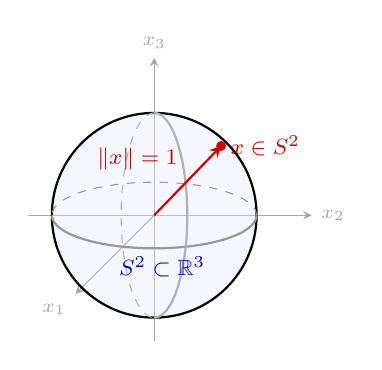
\begin{tikzpicture}[scale=1.0, >=stealth]
  % 3D axes
  \draw[->, gray!70] (-1.6, 0) -- (2.0, 0) node[right, font=\scriptsize] {$x_2$};
  \draw[->, gray!70] (0, -1.6) -- (0, 2.0) node[above, font=\scriptsize] {$x_3$};
  \draw[->, gray!70] (0,0) -- (-1.0, -1.0) node[below left, font=\scriptsize] {$x_1$};
  
  % Sphere
  \draw[thick, fill=blue!10, fill opacity=0.35] (0,0) circle (1.3);
  % Equator
  \draw[dashed, gray!80] (1.3,0) arc (0:180:1.3 and 0.42);
  \draw[thick, gray!80] (-1.3,0) arc (180:360:1.3 and 0.42);
  % Meridian
  \draw[dashed, gray!60] (0,1.3) arc (90:270:0.42 and 1.3);
  \draw[thick, gray!60] (0,1.3) arc (90:-90:0.42 and 1.3);
  
  % Point x on sphere and radius vector
  \draw[->, thick, red!80!black] (0,0) -- (0.85, 0.88) node[midway, above left, font=\footnotesize] {$\|x\|=1$};
  \fill[red!80!black] (0.85, 0.88) circle (1.8pt) node[right, font=\footnotesize] {$x \in S^2$};
  \node[font=\footnotesize, text=blue!80!black] at (0.1, -0.65) {$S^2 \subset \mathbb{R}^3$};
\end{tikzpicture}
}
        \caption{Earth modeled by the unit sphere.}
        \label{fig:slides-sphere}
      \end{figure}
    \end{column}
  \end{columns}
\end{frame}

\begin{frame}{A Flat Map of a Small Region}
  \begin{figure}
    \centering
    \resizebox{!}{0.61\textheight}{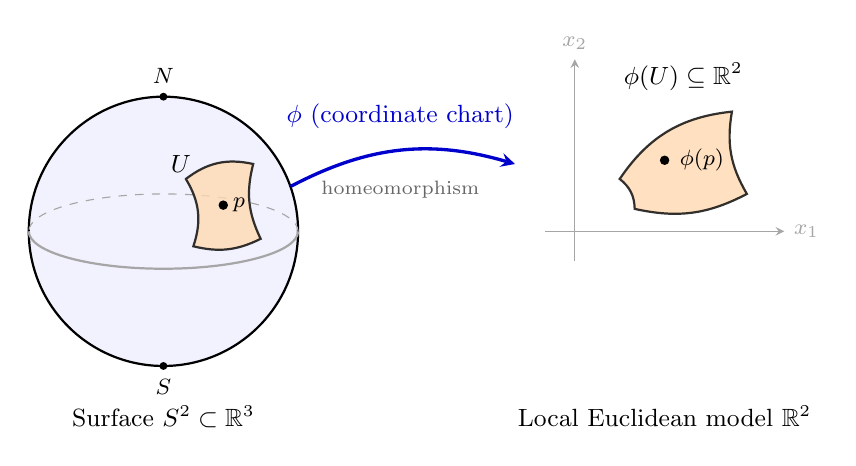
\begin{tikzpicture}[scale=0.95, >=stealth]
  % Left: Sphere S^2
  \begin{scope}[shift={(0,0)}]
    % Sphere outline
    \draw[thick, fill=blue!5] (0,0) circle (1.8);
    % Equator (front solid, back dashed)
    \draw[dashed, gray!70] (1.8,0) arc (0:180:1.8 and 0.5);
    \draw[thick, gray!70] (-1.8,0) arc (180:360:1.8 and 0.5);
    % North and South labels
    \node[above, font=\footnotesize] at (0, 1.85) {$N$};
    \fill (0,1.8) circle (1.5pt);
    \node[below, font=\footnotesize] at (0, -1.85) {$S$};
    \fill (0,-1.8) circle (1.5pt);

    % Local open patch U on sphere
    \draw[thick, fill=orange!30, opacity=0.8] 
      (0.3, 0.7) to[bend left=25] (1.2, 0.9) 
      to[bend right=20] (1.3, -0.1) 
      to[bend left=20] (0.4, -0.2) 
      to[bend right=25] cycle;
    \node[above left, font=\small] at (0.5, 0.65) {$U$};
    \fill (0.8, 0.35) circle (1.8pt) node[right, font=\footnotesize] {$p$};
    \node[below, font=\small] at (0, -2.2) {Surface $S^2 \subset \mathbb{R}^3$};
  \end{scope}

  % Middle: Coordinate chart map phi
  \draw[->, very thick, blue!80!black] (1.7, 0.6) to[bend left=22] 
    node[above=4pt, font=\small] {$\phi$ (coordinate chart)} 
    node[below=7pt, font=\scriptsize, text=gray!80!black] {homeomorphism} (4.7, 0.9);

  % Right: Flat open set in R^2
  \begin{scope}[shift={(5.5,0)}]
    % Axes - crossing at (0,0), clear of the region
    \draw[->, gray!70, thin] (-0.4, 0) -- (2.8, 0) node[right, font=\footnotesize] {$x_1$};
    \draw[->, gray!70, thin] (0, -0.4) -- (0, 2.3) node[above, font=\footnotesize] {$x_2$};
    
    % Flat open region phi(U) placed cleanly in the positive quadrant away from axes
    \draw[thick, fill=orange!30, opacity=0.8] 
      (0.6, 0.7) to[bend left=25] (2.1, 1.6) 
      to[bend right=20] (2.3, 0.5) 
      to[bend left=20] (0.8, 0.3) 
      to[bend right=25] cycle;
      
    % Region label placed comfortably above
    \node[above, font=\small] at (1.45, 1.75) {$\phi(U) \subseteq \mathbb{R}^2$};
    
    % Point phi(p) with label placed centered horizontally inside the orange patch
    \fill (1.2, 0.95) circle (1.8pt) node[right=2pt, font=\footnotesize] {$\phi(p)$};
    
    \node[below, font=\small] at (1.2, -2.2) {Local Euclidean model $\mathbb{R}^2$};
  \end{scope}
\end{tikzpicture}
}
    \caption{A surface region and its flat map.}
    \label{fig:slides-flat-map}
  \end{figure}
\end{frame}

\begin{frame}{Overlapping Maps of Nearby Regions}
  \begin{figure}
    \centering
    \resizebox{!}{0.59\textheight}{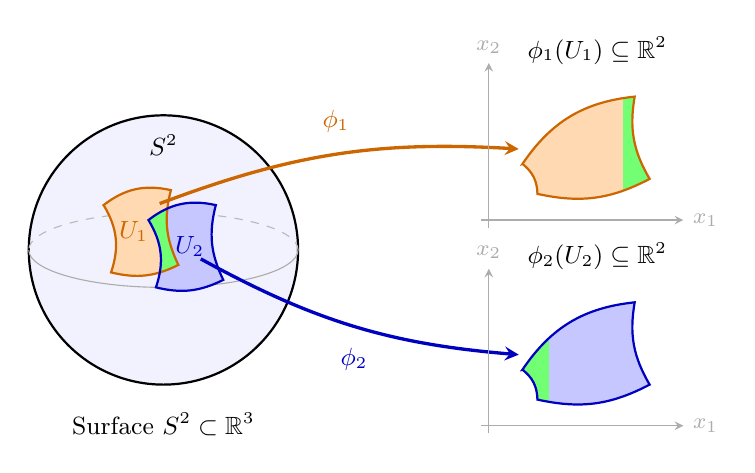
\begin{tikzpicture}[>=stealth, scale=0.95]
  % Reuse each boundary for its fill, overlap clipping, and outline.
  \def\surfacepatchone{(-0.8,0.6) to[bend left=25] (0.1,0.8)
    to[bend right=20] (0.2,-0.2) to[bend left=20] (-0.7,-0.3)
    to[bend right=25] cycle}
  \def\surfacepatchtwo{(-0.2,0.4) to[bend left=25] (0.7,0.6)
    to[bend right=20] (0.8,-0.4) to[bend left=20] (-0.1,-0.5)
    to[bend right=25] cycle}
  \def\flatpatch{(-0.8,-0.2) to[bend left=25] (0.7,0.7)
    to[bend right=20] (0.9,-0.4) to[bend left=20] (-0.6,-0.6)
    to[bend right=25] cycle}

  % Nearby irregular surface patches with a small shared region.
  \draw[thick, fill=blue!5] (0,0) circle (1.8);
  \draw[dashed, gray!55] (1.8,0) arc (0:180:1.8 and 0.5);
  \draw[gray!65] (-1.8,0) arc (180:360:1.8 and 0.5);
  \node[font=\small] at (0,1.4) {$S^2$};

  \fill[orange!30] \surfacepatchone;
  \fill[blue!22] \surfacepatchtwo;
  \begin{scope}
    \clip \surfacepatchone;
    \clip \surfacepatchtwo;
    \fill[green!55] (-1.0,-0.6) rectangle (1.2,1.0);
  \end{scope}
  \draw[thick, orange!80!black] \surfacepatchone;
  \draw[thick, blue!75!black] \surfacepatchtwo;
  \node[font=\small, text=orange!80!black] at (-0.4,0.25) {$U_1$};
  \node[font=\small, text=blue!75!black] at (0.35,0.05) {$U_2$};
  \node[below, font=\small] at (0,-2.05) {Surface $S^2\subset\mathbb{R}^3$};

  % Each patch has its own flat map, shown with two coordinate axes.
  \draw[->, very thick, orange!80!black]
    (-0.05,0.62) to[bend left=12]
    node[above=4pt, font=\small] {$\phi_1$} (4.75,1.35);
  \draw[->, very thick, blue!75!black]
    (0.5,-0.12) to[bend right=12]
    node[below=4pt, font=\small] {$\phi_2$} (4.75,-1.4);

  \begin{scope}[shift={(5.6,1.35)}]
    \draw[->, gray!65, thin] (-1.35,-0.95) -- (1.35,-0.95)
      node[right, font=\footnotesize] {$x_1$};
    \draw[->, gray!65, thin] (-1.25,-1.05) -- (-1.25,1.15)
      node[above, font=\footnotesize] {$x_2$};
    \fill[orange!30] \flatpatch;
    \begin{scope}
      \clip \flatpatch;
      \fill[green!55] (0.55,-0.8) rectangle (1.05,0.9);
    \end{scope}
    \draw[thick, orange!80!black] \flatpatch;
    \node[font=\small, above] at (0.2,1.0)
      {$\phi_1(U_1)\subseteq\mathbb{R}^2$};
  \end{scope}

  \begin{scope}[shift={(5.6,-1.4)}]
    \draw[->, gray!65, thin] (-1.35,-0.95) -- (1.35,-0.95)
      node[right, font=\footnotesize] {$x_1$};
    \draw[->, gray!65, thin] (-1.25,-1.05) -- (-1.25,1.15)
      node[above, font=\footnotesize] {$x_2$};
    \fill[blue!22] \flatpatch;
    \begin{scope}
      \clip \flatpatch;
      \fill[green!55] (-1.05,-0.8) rectangle (-0.45,0.9);
    \end{scope}
    \draw[thick, blue!75!black] \flatpatch;
    \node[font=\small, above] at (0.2,1.0)
      {$\phi_2(U_2)\subseteq\mathbb{R}^2$};
  \end{scope}
\end{tikzpicture}
}
    \caption{Overlapping maps: \textcolor{green!45!black}{green} marks the same shared region.}
    \label{fig:slides-overlapping-maps}
  \end{figure}
\end{frame}

\begin{frame}{Visualizing $S^2$ with Two Overlapping Patches}
  \begin{figure}
    \centering
    \resizebox{0.98\textwidth}{!}{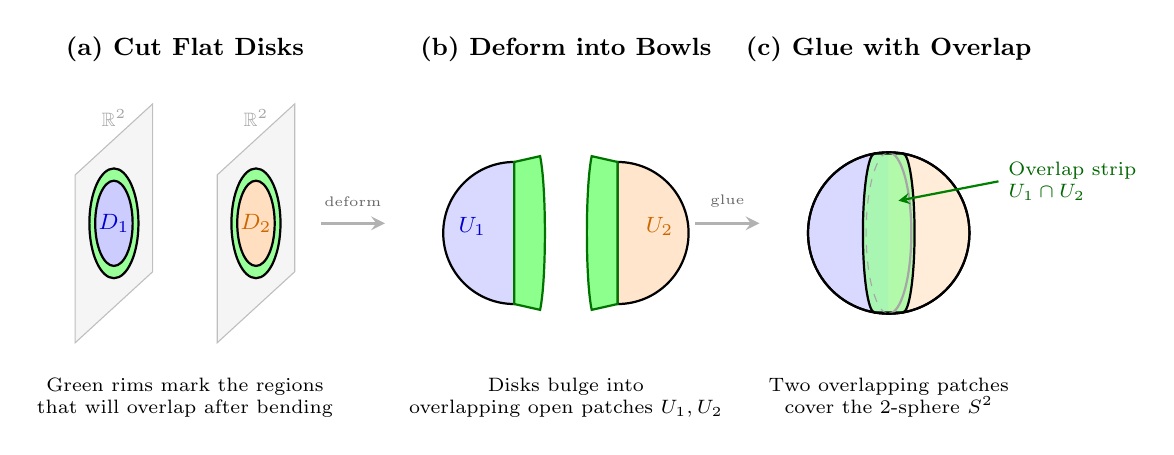
\begin{tikzpicture}[scale=0.82, >=stealth]
  % -------------------------------------------------------------
  % Panel 1: Cut two disks from parallel planes
  % -------------------------------------------------------------
  \begin{scope}[shift={(0,0)}]
    \node[above, font=\bfseries\small] at (1.3, 2.5) {(a) Cut Flat Disks};
    
    % Left plane
    \draw[gray!50, fill=gray!8] (-0.4, -1.7) -- (0.8, -0.6) -- (0.8, 2.0) -- (-0.4, 0.9) -- cycle;
    \node[above, gray!70, font=\scriptsize] at (0.2, 1.5) {$\mathbb{R}^2$};
    % Left disk with a green rim marking the future overlap collar
    \draw[thick, fill=green!40] (0.2, 0.15) ellipse (0.38 and 0.85);
    \draw[thick, fill=blue!20] (0.2, 0.15) ellipse (0.29 and 0.66);
    \node[font=\footnotesize, text=blue!80!black] at (0.2, 0.15) {$D_1$};
    \coordinate (chart-D1) at (0.55,0.15);

    % Right plane
    \draw[gray!50, fill=gray!8] (1.8, -1.7) -- (3.0, -0.6) -- (3.0, 2.0) -- (1.8, 0.9) -- cycle;
    \node[above, gray!70, font=\scriptsize] at (2.4, 1.5) {$\mathbb{R}^2$};
    % Right disk with a matching future overlap collar
    \draw[thick, fill=green!40] (2.4, 0.15) ellipse (0.38 and 0.85);
    \draw[thick, fill=orange!25] (2.4, 0.15) ellipse (0.29 and 0.66);
    \node[font=\footnotesize, text=orange!80!black] at (2.4, 0.15) {$D_2$};
    \coordinate (chart-D2) at (2.75,0.15);

    \node[below, font=\scriptsize, align=center] at (1.3, -2.1) {Green rims mark the regions\\that will overlap after bending};
  \end{scope}

  % Arrow 1 -> 2
  \draw[->, very thick, gray!60] (3.4, 0.15) -- (4.4, 0.15) node[midway, above=2pt, font=\tiny, text=gray!80!black] {deform};

  % -------------------------------------------------------------
  % Panel 2: Deform into overlapping open patches
  % -------------------------------------------------------------
  \begin{scope}[shift={(6.2,0)}]
    \node[above, font=\bfseries\small] at (1.0, 2.5) {(b) Deform into Bowls};

    % Surface strips match the patches in sphere_transition.tex.
    \draw[thick, fill=blue!15]
      (0.2, 1.1) arc (90:270:1.1 and 1.1) -- cycle;
    \path[fill=green!45, draw=green!45!black, thick]
      (0.2,1.1) -- (0.2,-1.1) -- (0.60,-1.19)
      .. controls (0.70,-0.73) and (0.70,0.73) .. (0.60,1.19) -- cycle;
    \node[font=\footnotesize, text=blue!80!black] at (-0.45, 0.1) {$U_1$};
    \coordinate (chart-U1) at (0.0,0.9);
    \coordinate (transition-U1) at (0.5,0.15);

    \draw[thick, fill=orange!20]
      (1.8, 1.1) arc (90:-90:1.1 and 1.1) -- cycle;
    \path[fill=green!45, draw=green!45!black, thick]
      (1.8,1.1) -- (1.8,-1.1) -- (1.40,-1.19)
      .. controls (1.30,-0.73) and (1.30,0.73) .. (1.40,1.19) -- cycle;
    \node[font=\footnotesize, text=orange!80!black] at (2.45, 0.1) {$U_2$};
    \coordinate (chart-U2) at (2.4,0.8);
    \coordinate (transition-U2) at (1.5,0.15);

    \node[below, font=\scriptsize, align=center] at (1.0, -2.1) {Disks bulge into\\overlapping open patches $U_1, U_2$};
  \end{scope}

  % Arrow 2 -> 3
  \draw[->, very thick, gray!60] (9.2, 0.15) -- (10.2, 0.15) node[midway, above=2pt, font=\tiny, text=gray!80!black] {glue};

  % -------------------------------------------------------------
  % Panel 3: Glued together with overlapping strip
  % -------------------------------------------------------------
  \begin{scope}[shift={(12.2,0)}]
    \node[above, font=\bfseries\small] at (0, 2.5) {(c) Glue with Overlap};

    % Left hemisphere (blue)
    \draw[thick, fill=blue!15] (0, 1.25) arc (90:270:1.25);
    
    % Right hemisphere (orange)
    \draw[thick, fill=orange!15] (0, 1.25) arc (90:-90:1.25);

    % Overlapping collar / strip in center (green tint)
    \draw[thick, fill=green!40, fill opacity=0.75] 
      (-0.22, 1.23) arc (90:270:0.18 and 1.23) 
      -- (0.22, -1.23) arc (-90:90:0.18 and 1.23) -- cycle;
      
    % Central boundary curve
    \draw[dashed, gray!70] (0, 1.25) arc (90:270:0.35 and 1.25);
    \draw[thick, gray!70] (0, 1.25) arc (90:-90:0.35 and 1.25);

    % Full sphere circle boundary
    \draw[thick] (0,0) circle (1.25);

    % Callout for overlap placed clearly outside the sphere to the right
    \draw[->, thick, green!50!black] (1.7, 0.8) -- (0.15, 0.5);
    \node[right, font=\scriptsize, align=left, text=green!40!black] at (1.7, 0.8) {Overlap strip\\$U_1 \cap U_2$};

    \node[below, font=\scriptsize, align=center] at (0, -2.1) {Two overlapping patches\\cover the 2-sphere $S^2$};
  \end{scope}

  % The chart-map slide enables these arrows; the original figure omits them.
  \ifdefined\showchartmaps
    \draw[->, very thick, blue!80!black]
      (chart-U1) .. controls +(-0.4,1.8) and +(0.8,2.4) .. (chart-D1)
      node[midway, above=4pt, font=\small] {$\phi_1$};
    \draw[->, very thick, orange!80!black,
        preaction={draw=white,line width=3.5pt}]
      (chart-U2) .. controls +(-1.0,1.9) and +(1.0,2.2) .. (chart-D2)
      node[midway, above=4pt, font=\small] {$\phi_2$};
  \fi

  % A separate variant traces one point through a coordinate transition.
  \ifdefined\showtransitionmaps
    \draw[->, very thick, blue!80!black, shorten <=3pt, shorten >=3pt]
      (chart-D1) .. controls +(0.9,2.2) and +(-0.2,2.2) .. (transition-U1)
      node[midway, above=4pt, font=\small] {$\phi_1^{-1}$};
    \draw[->, very thick, orange!80!black, shorten <=3pt, shorten >=3pt,
        preaction={draw=white,line width=3.5pt}]
      (transition-U2) .. controls +(-0.3,2.0) and +(1.0,2.4) .. (chart-D2)
      node[midway, above=4pt, font=\small] {$\phi_2$};
    \draw[densely dashed, thick, red!80!black, shorten <=4.5pt, shorten >=4.5pt]
      (transition-U1) -- (transition-U2);
    \draw[->, very thick, red!80!black, shorten <=3pt, shorten >=3pt]
      (chart-D1) .. controls +(0.3,-1.65) and +(0.6,-1.65) .. (chart-D2)
      node[midway, below=3pt, font=\small] {$\phi_2\circ\phi_1^{-1}$};
    \foreach \point in {chart-D1,transition-U1,transition-U2,chart-D2}
      \filldraw[fill=red!85!black,draw=white,line width=0.35pt]
        (\point) circle[radius=2.2pt];
    \node[below=10pt,font=\scriptsize,text=red!80!black] at (transition-U1) {$p$};
    \node[below=10pt,font=\scriptsize,text=red!80!black] at (transition-U2) {$p$};
  \fi
\end{tikzpicture}
}
    \caption{Two overlapping patches covering $S^2$.}
    \label{fig:slides-gluing-sphere}
  \end{figure}
\end{frame}

\begin{frame}{Smooth Manifolds: Coordinate Charts}
  \begin{definition}[Coordinate chart of dimension $n$]
    Let $M$ be a Hausdorff, second-countable topological space.
    A chart is a pair $(U,\phi)$ with $U\subseteq M$ open and
    \begin{equation}
      \label{eq:slides-coordinate-chart}
      \phi\colon U\longrightarrow\phi(U)\subseteq\mathbb{R}^n
    \end{equation}
    a homeomorphism onto an open subset of $\mathbb{R}^n$.
  \end{definition}
  \sources{\cite[Chapter~1, pp.~11--13]{lee2013smooth};
    \cite[Chapter~2]{tu2011introduction}.}
\end{frame}

\begin{frame}{Chart Maps in the Gluing Picture}
  \begin{figure}
    \centering
    \begingroup
      \def\showchartmaps{1}
      \resizebox{0.98\textwidth}{!}{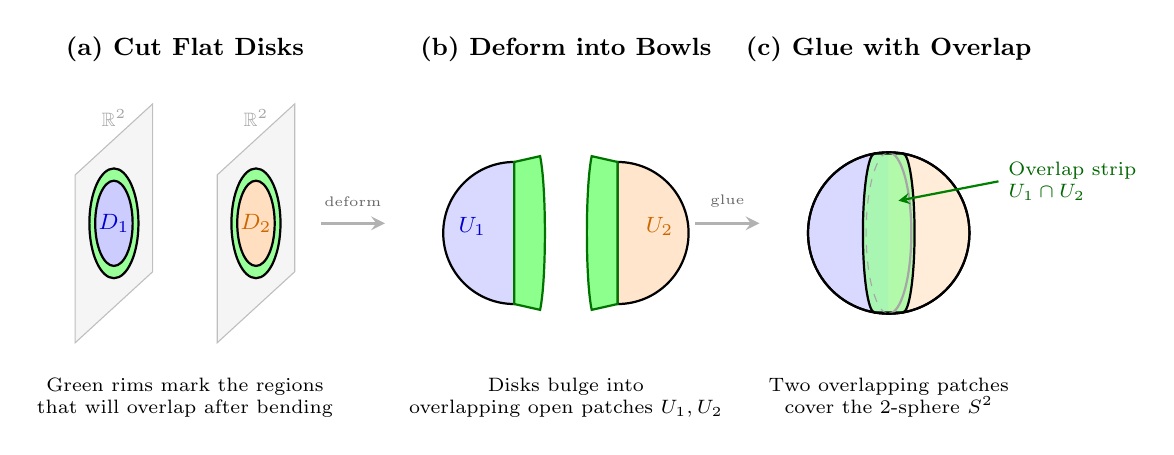
\begin{tikzpicture}[scale=0.82, >=stealth]
  % -------------------------------------------------------------
  % Panel 1: Cut two disks from parallel planes
  % -------------------------------------------------------------
  \begin{scope}[shift={(0,0)}]
    \node[above, font=\bfseries\small] at (1.3, 2.5) {(a) Cut Flat Disks};
    
    % Left plane
    \draw[gray!50, fill=gray!8] (-0.4, -1.7) -- (0.8, -0.6) -- (0.8, 2.0) -- (-0.4, 0.9) -- cycle;
    \node[above, gray!70, font=\scriptsize] at (0.2, 1.5) {$\mathbb{R}^2$};
    % Left disk with a green rim marking the future overlap collar
    \draw[thick, fill=green!40] (0.2, 0.15) ellipse (0.38 and 0.85);
    \draw[thick, fill=blue!20] (0.2, 0.15) ellipse (0.29 and 0.66);
    \node[font=\footnotesize, text=blue!80!black] at (0.2, 0.15) {$D_1$};
    \coordinate (chart-D1) at (0.55,0.15);

    % Right plane
    \draw[gray!50, fill=gray!8] (1.8, -1.7) -- (3.0, -0.6) -- (3.0, 2.0) -- (1.8, 0.9) -- cycle;
    \node[above, gray!70, font=\scriptsize] at (2.4, 1.5) {$\mathbb{R}^2$};
    % Right disk with a matching future overlap collar
    \draw[thick, fill=green!40] (2.4, 0.15) ellipse (0.38 and 0.85);
    \draw[thick, fill=orange!25] (2.4, 0.15) ellipse (0.29 and 0.66);
    \node[font=\footnotesize, text=orange!80!black] at (2.4, 0.15) {$D_2$};
    \coordinate (chart-D2) at (2.75,0.15);

    \node[below, font=\scriptsize, align=center] at (1.3, -2.1) {Green rims mark the regions\\that will overlap after bending};
  \end{scope}

  % Arrow 1 -> 2
  \draw[->, very thick, gray!60] (3.4, 0.15) -- (4.4, 0.15) node[midway, above=2pt, font=\tiny, text=gray!80!black] {deform};

  % -------------------------------------------------------------
  % Panel 2: Deform into overlapping open patches
  % -------------------------------------------------------------
  \begin{scope}[shift={(6.2,0)}]
    \node[above, font=\bfseries\small] at (1.0, 2.5) {(b) Deform into Bowls};

    % Surface strips match the patches in sphere_transition.tex.
    \draw[thick, fill=blue!15]
      (0.2, 1.1) arc (90:270:1.1 and 1.1) -- cycle;
    \path[fill=green!45, draw=green!45!black, thick]
      (0.2,1.1) -- (0.2,-1.1) -- (0.60,-1.19)
      .. controls (0.70,-0.73) and (0.70,0.73) .. (0.60,1.19) -- cycle;
    \node[font=\footnotesize, text=blue!80!black] at (-0.45, 0.1) {$U_1$};
    \coordinate (chart-U1) at (0.0,0.9);
    \coordinate (transition-U1) at (0.5,0.15);

    \draw[thick, fill=orange!20]
      (1.8, 1.1) arc (90:-90:1.1 and 1.1) -- cycle;
    \path[fill=green!45, draw=green!45!black, thick]
      (1.8,1.1) -- (1.8,-1.1) -- (1.40,-1.19)
      .. controls (1.30,-0.73) and (1.30,0.73) .. (1.40,1.19) -- cycle;
    \node[font=\footnotesize, text=orange!80!black] at (2.45, 0.1) {$U_2$};
    \coordinate (chart-U2) at (2.4,0.8);
    \coordinate (transition-U2) at (1.5,0.15);

    \node[below, font=\scriptsize, align=center] at (1.0, -2.1) {Disks bulge into\\overlapping open patches $U_1, U_2$};
  \end{scope}

  % Arrow 2 -> 3
  \draw[->, very thick, gray!60] (9.2, 0.15) -- (10.2, 0.15) node[midway, above=2pt, font=\tiny, text=gray!80!black] {glue};

  % -------------------------------------------------------------
  % Panel 3: Glued together with overlapping strip
  % -------------------------------------------------------------
  \begin{scope}[shift={(12.2,0)}]
    \node[above, font=\bfseries\small] at (0, 2.5) {(c) Glue with Overlap};

    % Left hemisphere (blue)
    \draw[thick, fill=blue!15] (0, 1.25) arc (90:270:1.25);
    
    % Right hemisphere (orange)
    \draw[thick, fill=orange!15] (0, 1.25) arc (90:-90:1.25);

    % Overlapping collar / strip in center (green tint)
    \draw[thick, fill=green!40, fill opacity=0.75] 
      (-0.22, 1.23) arc (90:270:0.18 and 1.23) 
      -- (0.22, -1.23) arc (-90:90:0.18 and 1.23) -- cycle;
      
    % Central boundary curve
    \draw[dashed, gray!70] (0, 1.25) arc (90:270:0.35 and 1.25);
    \draw[thick, gray!70] (0, 1.25) arc (90:-90:0.35 and 1.25);

    % Full sphere circle boundary
    \draw[thick] (0,0) circle (1.25);

    % Callout for overlap placed clearly outside the sphere to the right
    \draw[->, thick, green!50!black] (1.7, 0.8) -- (0.15, 0.5);
    \node[right, font=\scriptsize, align=left, text=green!40!black] at (1.7, 0.8) {Overlap strip\\$U_1 \cap U_2$};

    \node[below, font=\scriptsize, align=center] at (0, -2.1) {Two overlapping patches\\cover the 2-sphere $S^2$};
  \end{scope}

  % The chart-map slide enables these arrows; the original figure omits them.
  \ifdefined\showchartmaps
    \draw[->, very thick, blue!80!black]
      (chart-U1) .. controls +(-0.4,1.8) and +(0.8,2.4) .. (chart-D1)
      node[midway, above=4pt, font=\small] {$\phi_1$};
    \draw[->, very thick, orange!80!black,
        preaction={draw=white,line width=3.5pt}]
      (chart-U2) .. controls +(-1.0,1.9) and +(1.0,2.2) .. (chart-D2)
      node[midway, above=4pt, font=\small] {$\phi_2$};
  \fi

  % A separate variant traces one point through a coordinate transition.
  \ifdefined\showtransitionmaps
    \draw[->, very thick, blue!80!black, shorten <=3pt, shorten >=3pt]
      (chart-D1) .. controls +(0.9,2.2) and +(-0.2,2.2) .. (transition-U1)
      node[midway, above=4pt, font=\small] {$\phi_1^{-1}$};
    \draw[->, very thick, orange!80!black, shorten <=3pt, shorten >=3pt,
        preaction={draw=white,line width=3.5pt}]
      (transition-U2) .. controls +(-0.3,2.0) and +(1.0,2.4) .. (chart-D2)
      node[midway, above=4pt, font=\small] {$\phi_2$};
    \draw[densely dashed, thick, red!80!black, shorten <=4.5pt, shorten >=4.5pt]
      (transition-U1) -- (transition-U2);
    \draw[->, very thick, red!80!black, shorten <=3pt, shorten >=3pt]
      (chart-D1) .. controls +(0.3,-1.65) and +(0.6,-1.65) .. (chart-D2)
      node[midway, below=3pt, font=\small] {$\phi_2\circ\phi_1^{-1}$};
    \foreach \point in {chart-D1,transition-U1,transition-U2,chart-D2}
      \filldraw[fill=red!85!black,draw=white,line width=0.35pt]
        (\point) circle[radius=2.2pt];
    \node[below=10pt,font=\scriptsize,text=red!80!black] at (transition-U1) {$p$};
    \node[below=10pt,font=\scriptsize,text=red!80!black] at (transition-U2) {$p$};
  \fi
\end{tikzpicture}
}
    \endgroup
    \caption{Chart maps $\phi_1$ and $\phi_2$ reverse the disk-to-patch deformation.}
    \label{fig:slides-gluing-chart-maps}
  \end{figure}
\end{frame}

\begin{frame}{Smooth Manifolds: Compatible Charts}
  \begin{definition}[Coordinate chart of dimension $n$]
    Let $M$ be a Hausdorff, second-countable topological space.
    A chart is a pair $(U,\phi)$ with $U\subseteq M$ open and
    \begin{equation*}
      \tag{\ref{eq:slides-coordinate-chart}}
      \phi\colon U\longrightarrow\phi(U)\subseteq\mathbb{R}^n
    \end{equation*}
    a homeomorphism onto an open subset of $\mathbb{R}^n$.
  \end{definition}
  \begin{definition}[Smooth compatibility]
    Charts $(U,\phi)$ and $(V,\psi)$ are smoothly compatible if
    $U\cap V=\varnothing$, or
    \begin{equation}
      \psi\circ\phi^{-1}\colon\phi(U\cap V)\longrightarrow\psi(U\cap V)
    \end{equation}
    is a smooth diffeomorphism.
  \end{definition}
  \sources{\cite[Chapter~1, pp.~11--13]{lee2013smooth};
    \cite[Chapter~2]{tu2011introduction}.}
\end{frame}

\begin{frame}{The Transition Map on a Shared Point}
  \begin{figure}
    \centering
    \begingroup
      \def\showtransitionmaps{1}
      \resizebox{0.98\textwidth}{!}{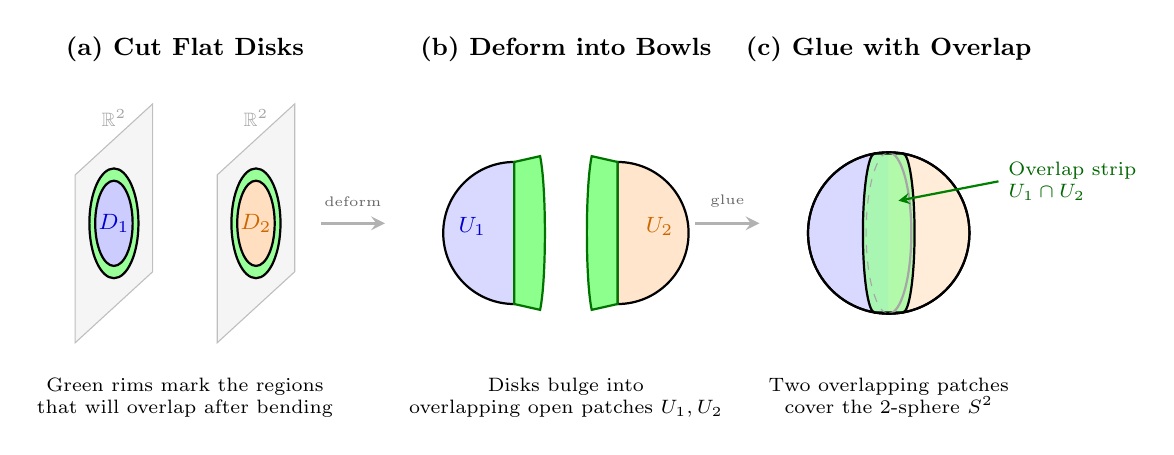
\begin{tikzpicture}[scale=0.82, >=stealth]
  % -------------------------------------------------------------
  % Panel 1: Cut two disks from parallel planes
  % -------------------------------------------------------------
  \begin{scope}[shift={(0,0)}]
    \node[above, font=\bfseries\small] at (1.3, 2.5) {(a) Cut Flat Disks};
    
    % Left plane
    \draw[gray!50, fill=gray!8] (-0.4, -1.7) -- (0.8, -0.6) -- (0.8, 2.0) -- (-0.4, 0.9) -- cycle;
    \node[above, gray!70, font=\scriptsize] at (0.2, 1.5) {$\mathbb{R}^2$};
    % Left disk with a green rim marking the future overlap collar
    \draw[thick, fill=green!40] (0.2, 0.15) ellipse (0.38 and 0.85);
    \draw[thick, fill=blue!20] (0.2, 0.15) ellipse (0.29 and 0.66);
    \node[font=\footnotesize, text=blue!80!black] at (0.2, 0.15) {$D_1$};
    \coordinate (chart-D1) at (0.55,0.15);

    % Right plane
    \draw[gray!50, fill=gray!8] (1.8, -1.7) -- (3.0, -0.6) -- (3.0, 2.0) -- (1.8, 0.9) -- cycle;
    \node[above, gray!70, font=\scriptsize] at (2.4, 1.5) {$\mathbb{R}^2$};
    % Right disk with a matching future overlap collar
    \draw[thick, fill=green!40] (2.4, 0.15) ellipse (0.38 and 0.85);
    \draw[thick, fill=orange!25] (2.4, 0.15) ellipse (0.29 and 0.66);
    \node[font=\footnotesize, text=orange!80!black] at (2.4, 0.15) {$D_2$};
    \coordinate (chart-D2) at (2.75,0.15);

    \node[below, font=\scriptsize, align=center] at (1.3, -2.1) {Green rims mark the regions\\that will overlap after bending};
  \end{scope}

  % Arrow 1 -> 2
  \draw[->, very thick, gray!60] (3.4, 0.15) -- (4.4, 0.15) node[midway, above=2pt, font=\tiny, text=gray!80!black] {deform};

  % -------------------------------------------------------------
  % Panel 2: Deform into overlapping open patches
  % -------------------------------------------------------------
  \begin{scope}[shift={(6.2,0)}]
    \node[above, font=\bfseries\small] at (1.0, 2.5) {(b) Deform into Bowls};

    % Surface strips match the patches in sphere_transition.tex.
    \draw[thick, fill=blue!15]
      (0.2, 1.1) arc (90:270:1.1 and 1.1) -- cycle;
    \path[fill=green!45, draw=green!45!black, thick]
      (0.2,1.1) -- (0.2,-1.1) -- (0.60,-1.19)
      .. controls (0.70,-0.73) and (0.70,0.73) .. (0.60,1.19) -- cycle;
    \node[font=\footnotesize, text=blue!80!black] at (-0.45, 0.1) {$U_1$};
    \coordinate (chart-U1) at (0.0,0.9);
    \coordinate (transition-U1) at (0.5,0.15);

    \draw[thick, fill=orange!20]
      (1.8, 1.1) arc (90:-90:1.1 and 1.1) -- cycle;
    \path[fill=green!45, draw=green!45!black, thick]
      (1.8,1.1) -- (1.8,-1.1) -- (1.40,-1.19)
      .. controls (1.30,-0.73) and (1.30,0.73) .. (1.40,1.19) -- cycle;
    \node[font=\footnotesize, text=orange!80!black] at (2.45, 0.1) {$U_2$};
    \coordinate (chart-U2) at (2.4,0.8);
    \coordinate (transition-U2) at (1.5,0.15);

    \node[below, font=\scriptsize, align=center] at (1.0, -2.1) {Disks bulge into\\overlapping open patches $U_1, U_2$};
  \end{scope}

  % Arrow 2 -> 3
  \draw[->, very thick, gray!60] (9.2, 0.15) -- (10.2, 0.15) node[midway, above=2pt, font=\tiny, text=gray!80!black] {glue};

  % -------------------------------------------------------------
  % Panel 3: Glued together with overlapping strip
  % -------------------------------------------------------------
  \begin{scope}[shift={(12.2,0)}]
    \node[above, font=\bfseries\small] at (0, 2.5) {(c) Glue with Overlap};

    % Left hemisphere (blue)
    \draw[thick, fill=blue!15] (0, 1.25) arc (90:270:1.25);
    
    % Right hemisphere (orange)
    \draw[thick, fill=orange!15] (0, 1.25) arc (90:-90:1.25);

    % Overlapping collar / strip in center (green tint)
    \draw[thick, fill=green!40, fill opacity=0.75] 
      (-0.22, 1.23) arc (90:270:0.18 and 1.23) 
      -- (0.22, -1.23) arc (-90:90:0.18 and 1.23) -- cycle;
      
    % Central boundary curve
    \draw[dashed, gray!70] (0, 1.25) arc (90:270:0.35 and 1.25);
    \draw[thick, gray!70] (0, 1.25) arc (90:-90:0.35 and 1.25);

    % Full sphere circle boundary
    \draw[thick] (0,0) circle (1.25);

    % Callout for overlap placed clearly outside the sphere to the right
    \draw[->, thick, green!50!black] (1.7, 0.8) -- (0.15, 0.5);
    \node[right, font=\scriptsize, align=left, text=green!40!black] at (1.7, 0.8) {Overlap strip\\$U_1 \cap U_2$};

    \node[below, font=\scriptsize, align=center] at (0, -2.1) {Two overlapping patches\\cover the 2-sphere $S^2$};
  \end{scope}

  % The chart-map slide enables these arrows; the original figure omits them.
  \ifdefined\showchartmaps
    \draw[->, very thick, blue!80!black]
      (chart-U1) .. controls +(-0.4,1.8) and +(0.8,2.4) .. (chart-D1)
      node[midway, above=4pt, font=\small] {$\phi_1$};
    \draw[->, very thick, orange!80!black,
        preaction={draw=white,line width=3.5pt}]
      (chart-U2) .. controls +(-1.0,1.9) and +(1.0,2.2) .. (chart-D2)
      node[midway, above=4pt, font=\small] {$\phi_2$};
  \fi

  % A separate variant traces one point through a coordinate transition.
  \ifdefined\showtransitionmaps
    \draw[->, very thick, blue!80!black, shorten <=3pt, shorten >=3pt]
      (chart-D1) .. controls +(0.9,2.2) and +(-0.2,2.2) .. (transition-U1)
      node[midway, above=4pt, font=\small] {$\phi_1^{-1}$};
    \draw[->, very thick, orange!80!black, shorten <=3pt, shorten >=3pt,
        preaction={draw=white,line width=3.5pt}]
      (transition-U2) .. controls +(-0.3,2.0) and +(1.0,2.4) .. (chart-D2)
      node[midway, above=4pt, font=\small] {$\phi_2$};
    \draw[densely dashed, thick, red!80!black, shorten <=4.5pt, shorten >=4.5pt]
      (transition-U1) -- (transition-U2);
    \draw[->, very thick, red!80!black, shorten <=3pt, shorten >=3pt]
      (chart-D1) .. controls +(0.3,-1.65) and +(0.6,-1.65) .. (chart-D2)
      node[midway, below=3pt, font=\small] {$\phi_2\circ\phi_1^{-1}$};
    \foreach \point in {chart-D1,transition-U1,transition-U2,chart-D2}
      \filldraw[fill=red!85!black,draw=white,line width=0.35pt]
        (\point) circle[radius=2.2pt];
    \node[below=10pt,font=\scriptsize,text=red!80!black] at (transition-U1) {$p$};
    \node[below=10pt,font=\scriptsize,text=red!80!black] at (transition-U2) {$p$};
  \fi
\end{tikzpicture}
}
    \endgroup
    \caption{The same point $p$ in the overlap is marked in both patches; the
      composite transition map sends its image in $D_1$ to its image in $D_2$.}
    \label{fig:slides-transition-point}
  \end{figure}
\end{frame}

\begin{frame}{Smooth Manifolds: Atlases and the Definition}
  \begin{definition}[Smooth atlas of dimension $n$]
    A collection $\mathcal{A}=\{(U_\alpha,\phi_\alpha)\}_{\alpha\in I}$
    of smoothly compatible charts of dimension $n$ whose domains cover $M$:
    \begin{equation}
      \bigcup_{\alpha\in I}U_\alpha=M.
    \end{equation}
  \end{definition}
  \begin{definition}[Smooth $n$-manifold]
    A Hausdorff, second-countable topological space $M$ equipped with a
    smooth atlas of dimension $n$.
  \end{definition}
  Euclidean space $\mathbb{R}^n$, with its standard topology and identity chart,
  is a smooth $n$-manifold.
  \sources{\cite[pp.~11--13; Proposition~1.17, p.~13]{lee2013smooth}.}
\end{frame}

% Detailed sphere explanations and the benefits discussion remain spoken;
% the chart-map figure provides the visual link immediately after its definition.

\slidetitlesection{Tangent and Cotangent Spaces}

\begin{frame}{Tangent Directions on the Sphere}
  \begin{columns}[c,onlytextwidth]
    \begin{column}{0.43\textwidth}
      \begin{equation}
        p\in S^2,\qquad v\in\mathbb{R}^3,\qquad v\ne0.
      \end{equation}
      The vector $v$ lies in the geometric tangent plane at $p$.
      \begin{block}{The straight line leaves the sphere}
        \begin{equation}
          p+tv\notin S^2\qquad(t\ne0).
        \end{equation}
      \end{block}
    \end{column}
    \begin{column}{0.53\textwidth}
      \begin{figure}
        \centering
        \resizebox{0.91\linewidth}{!}{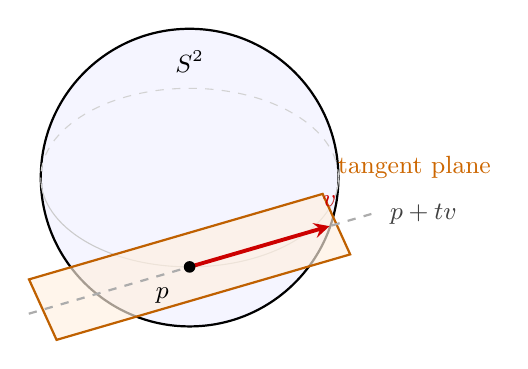
\begin{tikzpicture}[>=stealth, scale=1.05,
    x={(1.8cm,0cm)}, y={(0cm,1.44cm)}, z={(0cm,-1.08cm)}]
  % Use the same sphere projection as the curve-velocity figure.
  \draw[thick, fill=blue!4] (0,0) circle[radius=1.8cm];
  \draw[gray!35, dashed] (1.8cm,0cm) arc (0:180:1.8cm and 1.08cm);
  \draw[gray!40] (-1.8cm,0cm) arc (180:360:1.8cm and 1.08cm);
  \node[font=\small] at (0cm,1.4cm) {$S^2$};

  % The affine plane z=1 is tangent at p=(0,0,1).
  \filldraw[fill=orange!12, fill opacity=0.65,
      draw=orange!75!black, thick]
    (-0.894,-0.613,1) -- (1.079,0.105,1) --
    (0.894,0.613,1) -- (-1.079,-0.105,1) -- cycle;
  \node[font=\small, text=orange!80!black, above right=2pt]
    at (0.894,0.613,1) {tangent plane};

  % The tangent line lies in the plane and leaves the sphere away from p.
  \draw[gray!65, dashed, thick]
    ({-1.15*cos(20)},{-1.15*sin(20)},1) --
    ({1.30*cos(20)},{1.30*sin(20)},1)
    node[right=3pt, font=\small, text=black!75] {$p+tv$};
  \draw[->, red!80!black, line width=1.4pt]
    (0,0,1) -- ({cos(20)},{sin(20)},1)
    node[above=3pt, font=\small] {$v$};
  \fill (0,0,1) circle[radius=2pt];
  \node[font=\small, below left=4pt] at (0,0,1) {$p$};
\end{tikzpicture}
}
        \caption{A tangent direction and the line $p+tv$.}
        \label{fig:slides-tangent-direction}
      \end{figure}
    \end{column}
  \end{columns}
\end{frame}

\begin{frame}{Curves and Directional Derivatives}
  A smooth curve through $p$:
  \begin{equation}
    \gamma\colon(-\epsilon,\epsilon)\to M,\qquad\gamma(0)=p.
  \end{equation}
  For a smooth function $f\colon M\to\mathbb{R}$,
  \begin{equation}
    f\circ\gamma\colon(-\epsilon,\epsilon)\to\mathbb{R},
    \qquad t\mapsto f(\gamma(t)),
  \end{equation}
  with rate of change
  \begin{equation}
    \left.\frac{d}{dt}\right|_{t=0}f(\gamma(t)).
  \end{equation}
  \begin{example}[Euclidean space]
    For $M=\mathbb{R}^n$ and $\gamma(t)=p+tv$,
    \begin{equation}
      \left.\frac{d}{dt}\right|_{t=0}f(\gamma(t))
      =\left.\frac{d}{dt}\right|_{t=0}f(p+tv)=D_vf(p).
    \end{equation}
  \end{example}
\end{frame}

\begin{frame}{Different Curves, the Same Initial Velocity}
  \begin{figure}
    \centering
    \resizebox{!}{0.62\textheight}{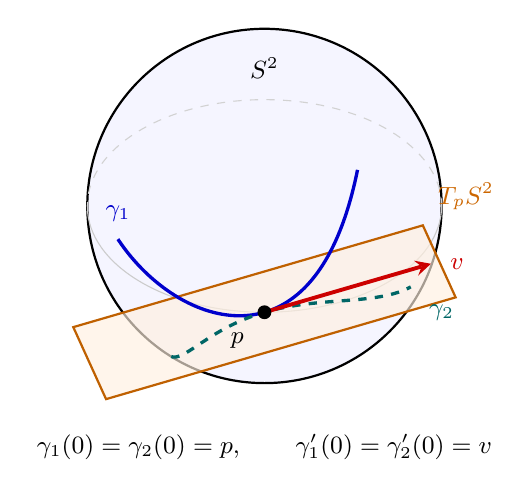
\begin{tikzpicture}[>=stealth, scale=1.25,
    x={(1.8cm,0cm)}, y={(0cm,1.44cm)}, z={(0cm,-1.08cm)}]
  % Orthographic projection of the unit sphere: (x,y,z) -> (1.8x,1.44y-1.08z).
  \draw[thick, fill=blue!4] (0,0) circle[radius=1.8cm];
  \draw[gray!35, dashed] (1.8cm,0cm) arc (0:180:1.8cm and 1.08cm);
  \draw[gray!40] (-1.8cm,0cm) arc (180:360:1.8cm and 1.08cm);
  \node[font=\small] at (0cm,1.4cm) {$S^2$};

  % A patch of the actual tangent plane z=1 at p=(0,0,1).
  \filldraw[fill=orange!12, fill opacity=0.65,
      draw=orange!75!black, thick]
    (-0.894,-0.613,1) -- (1.079,0.105,1) --
    (0.894,0.613,1) -- (-1.079,-0.105,1) -- cycle;
  \node[font=\small, text=orange!80!black, above right=2pt]
    at (0.894,0.613,1) {$T_pS^2$};

  % In a rotated tangent basis e1,e2, use
  % gamma_i(t)=t e1 +/- 0.85 t^2 e2 + sqrt(1-t^2-0.85^2 t^4) p.
  % Both lie on S^2, pass through p, and have derivative e1 at t=0.
  \draw[blue!80!black, very thick]
    plot[domain=-0.72:0.72, samples=101, variable=\t]
    ({cos(20)*\t-sin(20)*0.85*\t*\t},
     {sin(20)*\t+cos(20)*0.85*\t*\t},
     {sqrt(1-\t*\t-0.85*0.85*\t*\t*\t*\t)});
  \draw[teal!80!black, very thick, dashed]
    plot[domain=-0.72:0.72, samples=101, variable=\t]
    ({cos(20)*\t+sin(20)*0.85*\t*\t},
     {sin(20)*\t-cos(20)*0.85*\t*\t},
     {sqrt(1-\t*\t-0.85*0.85*\t*\t*\t*\t)});

  % Labels sit beside separated portions of the curves.
  \node[font=\small, text=blue!80!black, above=3pt]
    at (-0.827,0.168,0.537) {$\gamma_1$};
  \node[font=\small, text=teal!80!black, below right=3pt]
    at (0.827,-0.168,0.537) {$\gamma_2$};

  \draw[->, red!80!black, line width=1.4pt]
    (0,0,1) -- ({cos(20)},{sin(20)},1)
    node[right=3pt, font=\small] {$v$};
  \fill (0,0,1) circle[radius=2pt];
  \node[font=\small, below left=4pt] at (0,0,1) {$p$};
  \node[font=\small, align=center] at (0cm,-2.45cm)
    {$\gamma_1(0)=\gamma_2(0)=p,\qquad
       \gamma_1'(0)=\gamma_2'(0)=v$};
\end{tikzpicture}
}
    \caption{Curves with the same initial velocity represent the same tangent vector.}
    \label{fig:slides-curve-velocity}
  \end{figure}
  \sources{\cite[p.~72]{lee2013smooth}.}
\end{frame}

\begin{frame}{Tangent Vectors and Tangent Spaces}
  Let $M$ be a smooth $n$-manifold and $p\in M$.
  Let $\gamma_1\colon(-\epsilon,\epsilon)\to M$ and
  $\gamma_2\colon(-\epsilon,\epsilon)\to M$ be smooth curves with
  $\gamma_1(0)=\gamma_2(0)=p$.
  They are equivalent if, for every smooth function
  $f\colon M\to\mathbb{R}$,
  \begin{equation}
    \gamma_1\sim\gamma_2
    \quad\Longleftrightarrow\quad
    \left.\frac{d}{dt}\right|_{t=0}f(\gamma_1(t))
    =\left.\frac{d}{dt}\right|_{t=0}f(\gamma_2(t)).
  \end{equation}
  \begin{definition}
    A \textbf{tangent vector} at $p$ is an equivalence class $v=[\gamma]$.
    The \textbf{tangent space} is
    \begin{equation}
      T_pM=\{[\gamma]\mid\gamma\text{ is a smooth curve through }p\}.
    \end{equation}
  \end{definition}
  \begin{equation}
    \dim T_pM=n,
    \qquad T_p\mathbb{R}^n\cong\mathbb{R}^n,
    \qquad v\longleftrightarrow[t\mapsto p+tv].
  \end{equation}
  \sources{\cite[p.~72; Problem~3-8, p.~76; Proposition~3.10, p.~57]{lee2013smooth}.}
\end{frame}

\begin{frame}{Cotangent Vectors and Cotangent Spaces}
  \begin{definition}
    A \textbf{cotangent vector} at $p$ is a linear map $T_pM\to\mathbb{R}$.
    The \textbf{cotangent space} is
    \begin{equation}
      T_p^*M=\operatorname{Hom}_{\mathbb{R}}(T_pM,\mathbb{R}).
    \end{equation}
  \end{definition}
  \begin{example}[The differential of a smooth function]
    For a smooth function $f\colon M\to\mathbb{R}$ and a smooth curve
    $\gamma\colon(-\epsilon,\epsilon)\to M$ with $\gamma(0)=p$,
    \begin{equation}
      df_p\colon T_pM\to\mathbb{R},
      \qquad
      df_p([\gamma])=\left.\frac{d}{dt}\right|_{t=0}f(\gamma(t)).
    \end{equation}
  \end{example}
  \sources{\cite[Chapter~11]{lee2013smooth}.}
\end{frame}

\begin{frame}{The Differential and the Euclidean Gradient}
  Under $T_p\mathbb{R}^n\cong\mathbb{R}^n$, the gradient defines a linear map
  \begin{equation}
    \nabla f(p)\cdot(-)\colon\mathbb{R}^n\to\mathbb{R},
    \qquad v\mapsto\nabla f(p)\cdot v.
  \end{equation}
  For the straight-line curve $\gamma(t)=p+tv$,
  \begin{equation}
    df_p([\gamma])
    =\left.\frac{d}{dt}\right|_{t=0}f(p+tv)
    =\nabla f(p)\cdot v.
  \end{equation}
  \begin{block}{The same linear measurement}
    \begin{equation}
      df_p=\nabla f(p)\cdot(-).
    \end{equation}
  \end{block}
  \sources{\cite[Chapter~11]{lee2013smooth}.}
\end{frame}

\slidetitlesection{Differential Forms and the Exterior Derivative}

\begin{frame}{Differential $1$-Forms}
  \begin{definition}
    A \textbf{differential $1$-form} $\omega$ on $M$ assigns a cotangent vector
    $\omega_p\in T_p^*M$ to each $p\in M$, varying smoothly with $p$:
    \begin{equation}
      \omega_p\colon T_pM\longrightarrow\mathbb{R}.
    \end{equation}
  \end{definition}
  \begin{example}
    The differentials of a smooth function $f\colon M\to\mathbb{R}$ form a
    $1$-form:
    \begin{equation}
      df\colon p\longmapsto df_p.
    \end{equation}
  \end{example}
  \begin{equation}
    \underbrace{df_p}_{\text{at one point}}
    \qquad\qquad
    \underbrace{df}_{\text{on the whole manifold}}.
  \end{equation}
  \sources{\cite[p.~360]{lee2013smooth}; an integration-first perspective:
    \cite{tao2007differential}.}
\end{frame}

\begin{frame}{Vector Fields and $1$-Forms in Euclidean Space}
  \begin{example}[Start with the differential]
    For a smooth function $f\colon\mathbb{R}^n\to\mathbb{R}$ and
    $p\in\mathbb{R}^n$,
    \begin{equation}
      df_p(v)=\nabla f(p)\cdot v,
      \qquad v\in T_p\mathbb{R}^n=\mathbb{R}^n.
    \end{equation}
    The dot product with $\nabla f(p)$ gives $df_p$; across all points,
    $df$ corresponds to $\nabla f$.
  \end{example}
  \begin{block}{Generalize to any smooth vector field}
    For a smooth vector field $F$ on $\mathbb{R}^n$, define at each
    $p\in\mathbb{R}^n$:
    \begin{equation}
      \begin{aligned}
        (\omega_F)_p&\colon T_p\mathbb{R}^n=\mathbb{R}^n\longrightarrow\mathbb{R},\\
        (\omega_F)_p(v)&=F(p)\cdot v,
        \qquad v\in T_p\mathbb{R}^n=\mathbb{R}^n.
      \end{aligned}
    \end{equation}
  \end{block}
  Taking $F=\nabla f$ recovers $\omega_{\nabla f}=df$.
  \sources{\cite[Chapter~11; Equation~(14.27), p.~368]{lee2013smooth}.}
\end{frame}

\begin{frame}{Geometric Motivation for Higher Forms}
  A $2$-form gives a signed measurement of the parallelogram spanned by
  $v,w\in T_pM$.
  \begin{equation}
    \omega_p(v,w)=-\omega_p(w,v).
  \end{equation}
  Swapping the two vectors changes the sign, as in a cross product.
  \sources{\cite[Chapter~14]{lee2013smooth}.}
\end{frame}

\begin{frame}{Multilinear and Alternating Maps}
  \begin{definition}
    Let $V$ be a real vector space and
    \begin{equation}
      T\colon\underbrace{V\times\cdots\times V}_{k\text{ copies}}
      \longrightarrow\mathbb{R}.
    \end{equation}
    $T$ is \textbf{multilinear} if it is linear in each argument with the others fixed.

    \medskip
    It is \textbf{alternating} if swapping any two inputs changes its sign;
    i.e., for all $1\le i<j\le k$, we have
    \begin{equation}
      T(v_1,\ldots,v_i,\ldots,v_j,\ldots,v_k)
      =-T(v_1,\ldots,v_j,\ldots,v_i,\ldots,v_k).
    \end{equation}
  \end{definition}
  \sources{\cite[\S26, p.~220; \S27, pp.~229--230]{munkres1991analysis}.}
\end{frame}

\begin{frame}{Higher Differential Forms: At a Point and Globally}
  \begin{definition}[$k$-form at a point]
    An alternating multilinear map
    \begin{equation}
      \omega_p\colon
      \underbrace{T_pM\times\cdots\times T_pM}_{k\text{ copies}}
      \longrightarrow\mathbb{R}.
    \end{equation}
  \end{definition}
  \begin{definition}[Differential $k$-form on $M$]
    A smooth choice of a $k$-form $\omega_p$ at each $p\in M$.
  \end{definition}
  \begin{equation}
    \Omega^k(M)=\{\text{smooth differential }k\text{-forms on }M\},
    \qquad \Omega^0(M)=\{\text{smooth functions }M\to\mathbb{R}\}.
  \end{equation}
  \sources{\cite[``Differential Forms on Manifolds,'' pp.~359--360]{lee2013smooth}.}
\end{frame}

\begin{frame}{The Vector Space of Differential Forms}
  For $\omega,\omega'\in\Omega^k(M)$, $a\in\mathbb{R}$, and
  $v_1,\ldots,v_k\in T_pM$,
  \begin{equation}
    (\omega+\omega')_p(v_1,\ldots,v_k)
    =\omega_p(v_1,\ldots,v_k)+\omega'_p(v_1,\ldots,v_k).
  \end{equation}
  \begin{equation}
    (\omega+\omega')_p=\omega_p+\omega'_p,
    \qquad (a\omega)_p=a\omega_p.
  \end{equation}
  Smoothness, multilinearity, and alternation are preserved.
  \begin{equation}
    \Omega^k(M)\text{ is a real vector space}.
  \end{equation}
  \sources{\cite[p.~360]{lee2013smooth}.}
\end{frame}

\begin{frame}{The Exterior Derivative}
  \begin{definition}
    The \textbf{exterior derivative} is a linear operator
    \begin{equation}
      d\colon\Omega^k(M)\longrightarrow\Omega^{k+1}(M).
    \end{equation}
  \end{definition}
  \begin{block}{Properties}
    \begin{enumerate}
      \item \textbf{Linearity:}
        $d(a\alpha+b\beta)=a\,d\alpha+b\,d\beta$.
      \item \textbf{On functions:} $df$ is the differential of $f$.
      \item \textbf{Differentiating twice:}
        \begin{equation}
          d(d\omega)=0,\qquad d^2=0.
        \end{equation}
    \end{enumerate}
  \end{block}
  \sources{\cite[Theorem~14.24, pp.~365--366]{lee2013smooth}.}
\end{frame}

\begin{frame}{Exterior Derivatives and Vector Calculus on $\mathbb{R}^3$}
  \begin{equation}
    \begin{aligned}
      d&\colon\{\text{smooth }f\colon\mathbb{R}^3\to\mathbb{R}\}
        \to\Omega^1(\mathbb{R}^3)
        &&\text{gradient},\\
      d&\colon\Omega^1(\mathbb{R}^3)\to\Omega^2(\mathbb{R}^3)
        &&\text{curl},\\
      d&\colon\Omega^2(\mathbb{R}^3)\to\Omega^3(\mathbb{R}^3)
        &&\text{divergence}.
    \end{aligned}
  \end{equation}
  \begin{equation}
    \Omega^4(\mathbb{R}^3)=\{0\},
    \qquad d\colon\Omega^3(\mathbb{R}^3)\to\{0\}.
  \end{equation}
  \begin{block}{The familiar identities are instances of $d^2=0$}
    \begin{equation}
      \operatorname{curl}(\nabla f)=0,
      \qquad\operatorname{div}(\operatorname{curl}F)=0.
    \end{equation}
  \end{block}
  \sources{\cite[Equation~(14.27), p.~368; Exercise~14.28]{lee2013smooth};
    \cite[\S4.4.1, Table~4.4.8]{bouchard_exterior_vector}.}
\end{frame}

\slidetitlesection{de Rham Cohomology and Its Significance}

\begin{frame}{Cohomology Groups}
  For $\omega\in\Omega^k(M)$:
  \begin{equation}
    \omega\text{ is closed}\iff d\omega=0,
    \qquad
    \omega\text{ is exact}\iff\omega=d\eta
    \text{ for some }\eta\in\Omega^{k-1}(M).
  \end{equation}
  \begin{definition}[de Rham cohomology]
    For $k\ge0$,
    \begin{equation}
      H^k_{\mathrm{dR}}(M)
      =\frac{\{\text{closed }k\text{-forms on }M\}}
            {\{\text{exact }k\text{-forms on }M\}}
      =\frac{\ker\!\left(d\colon\Omega^k(M)\to\Omega^{k+1}(M)\right)}
            {\operatorname{im}\!\left(d\colon\Omega^{k-1}(M)\to\Omega^k(M)\right)}.
    \end{equation}
  \end{definition}
  Since $d^2=0$, every exact form is closed.
  \hfill{\small $\Omega^{-1}(M)=\{0\}$.}
  \sources{\cite[p.~441]{lee2013smooth}.}
\end{frame}

% Sphere cohomology remains optional in the manuscript and is not part of this deck.

\begin{frame}{The de Rham Theorem}
  \begin{theorem}[de Rham]
    For every smooth manifold $M$ and every integer $k\ge0$, there is a natural
    isomorphism of real vector spaces
    \begin{equation}
      H^k_{\mathrm{dR}}(M)\cong H^k(M;\mathbb{R}).
    \end{equation}
    Here $H^k(M;\mathbb{R})$ is singular cohomology with real coefficients,
    defined from the topology of $M$ alone.
  \end{theorem}
  \sources{\cite[Proposition~18.13, pp.~482--483; Theorem~18.14, p.~484]{lee2013smooth}.}
\end{frame}

\begin{frame}{Conservative Vector Fields and Topology}
  \begin{theorem}[Conservative vector fields]
    On a simply connected domain $X\subseteq\mathbb{R}^3$, a smooth vector
    field $F$ satisfies $\operatorname{curl}F=0$ if and only if $F=\nabla f$
    for some smooth function $f\colon X\to\mathbb{R}$.
  \end{theorem}
  \begin{proof}
  \setlength{\abovedisplayskip}{5pt}
  \setlength{\belowdisplayskip}{3pt}
  \begin{equation}
    H^1(X;\mathbb{R})=0
    \quad\xRightarrow{\text{de Rham}}\quad H^1_{\mathrm{dR}}(X)=0.
  \end{equation}
  \begin{equation}
    \Longrightarrow\quad
    \ker\!\left(d\colon\Omega^1(X)\to\Omega^2(X)\right)
    =\operatorname{im}\!\left(d\colon\Omega^0(X)\to\Omega^1(X)\right).
  \end{equation}
  For a smooth vector field $F$ and its associated $1$-form $\omega_F$,
  \begin{equation}
    \begin{aligned}
      \operatorname{curl}F=0 &\quad\Longleftrightarrow\quad d\omega_F=0
        \quad\Longrightarrow\quad \omega_F\in\ker d=\operatorname{im}d\\
        &\quad\Longrightarrow\quad
          \exists\text{ smooth }f\colon X\to\mathbb{R}:\ \omega_F=df.
    \end{aligned}
  \end{equation}
  \end{proof}
  \sources{\cite[Corollary~16.27, p.~421; p.~472; Problem~18-2, p.~487]{lee2013smooth}.}
\end{frame}

\begin{frame}[allowframebreaks,noframenumbering]{References}
  \scriptsize
  \bibliographystyle{alpha}
  \bibliography{../references}
\end{frame}

\begin{frame}[noframenumbering]{Acknowledgments}
  AI was used in typesetting and structuring the manuscript and presentation
  slides. Every part of the mathematics is written by hand.
\end{frame}

\end{document}
